\documentclass[9pt,aspectratio=169]{beamer}
\usetheme{VK}
\usepackage{subfig} % side by side logos
\usepackage{dsfont}
\usepackage{bm}
\usepackage{xunicode}
\usepackage{xltxtra}
\usepackage{xecyr}

\usepackage{tikz}
\usetikzlibrary{angles,quotes, shapes.geometric, shapes, arrows}

\usepackage{mwe}
\usepackage{multirow}

\usepackage{mathtools} % \mathclap for shortening overbrace text
\usepackage{bbm} % For indicator - \mathbbm{1}
\usepackage{soul} % to get \ul which underlines and allows text to wrap

\usepackage{csquotes}
\usepackage[style=verbose-ibid,backend=bibtex]{biblatex}
\bibliography{references}

%\date[]{}
\title[]{Title of Presentation}
\author[]{Your Name}
\date[]{Date of Presentation}

\AtEndDocument{\usebeamertemplate{endpage}}

\begin{document}
\maketitle

\begin{frame}{Introductory Frame Title}
    \begin{columns}
    \column{0.3\textwidth}
        Please enjoy the numbers presented on the right.
    \column{0.6\textwidth}
        \begin{tabular}{l l}
            \dblock{42}{Answer to everything} & \dblock{18}{Covid minus one} \\[2cm]
            \dblock{$\bm{\infty}$}{Cool ideas} & \dblock{1}{Fearless leader}
        \end{tabular}
    \end{columns}
    
\end{frame}

\begin{frame}{Flowchart/Outline Slide}
\ddef{Problem Context}{Describe the context of your work here.}
\begin{center} \arrowdown \end{center}
\vspace{-2mm}
\ddef{Solution}{Briefly describe the solution that your work provides here.}
\begin{center} \arrowdown \end{center}
\vspace{-2mm}
\ddef{Implication}{Describe the broader implications of your research here.}
\end{frame}

{
\setbeamercolor{background canvas}{bg=VKblue}
\begin{frame}[plain,noframenumbering]
\vspace{1cm}
\usebeamerfont{title}\usebeamercolor[fg]{title} \textbf{{\Huge Topic \#1}}    
\end{frame}
}

\begin{frame}{Fancy equation with colored highlights\\and notation}
\only<1>{
    \textbf{This is a linear model:}
   {\Huge $${\color{red}\overbrace{R}^{\mathclap{\substack{\text{{\small Description}} \\ \text{{\small here}}}}}} = \beta_0 + \beta_1{\color{purple}\overbrace{X}^{\mathclap{\text{{\small Description}}}}} + \beta_2{\color{blue}\overbrace{A}^{\mathclap{\text{{\small{Math:} $\{-1,1\}$}}}}} \phantom{+\beta_3\underbrace{AX}_{\mathclap{\text{{\small Interaction}}}}} +\epsilon$$} % see https://tex.stackexchange.com/questions/333744/a-more-beautiful-output-of-under-and-overbrace
   
   \begin{itemize}
       \item This is my takeaway from the linear model
       \begin{itemize}
           \item This is my sub-takeaway from the linear model
       \end{itemize}
    %   \par\noindent\phantom{\parbox{\linewidth}{ % see https://tex.stackexchange.com/questions/229411/can-i-use-phantom-to-hide-a-latex-environment-itemize
    %   \item test
    %   \begin{itemize}
    %       \item test
    %       \item test
    %   \end{itemize}}}\par
   \end{itemize}
   }
\only<2>{
    \textbf{This is a linear model with interaction:}
   {\Huge $${\color{red}\overbrace{R}^{\mathclap{\substack{\text{{\small Description}} \\ \text{{\small here}}}}}} = \beta_0 + \beta_1{\color{purple}\overbrace{X}^{\mathclap{\text{{\small Description}}}}} + \beta_2{\color{blue}\overbrace{A}^{\mathclap{\text{{\small{Math:} $\{-1,1\}$}}}}} +{\color{orange}\underbrace{\beta_3AX}_{\mathclap{\text{{\small Description}}}}} +\epsilon$$}
   
   \begin{itemize}
       \item Now, here is my takeaway from the interaction model
       \begin{itemize}
           \item Here is my sub-takeaway from the interaction model
       \end{itemize}
   \end{itemize}
   }
\end{frame}

\begin{frame}{\hypertarget{notation}{Notation and Definitions}}
\begin{itemize}
    \item Define something here
    \vspace{1mm}
    \begin{itemize}\setlength\itemsep{1mm}
        \item This is what $X$ represents
        \item This is what $A$ represents
        \item This is what $R$ represents
    \end{itemize}
    \item Define something else here
    \item Define something else here
    %\item Vectors and matrices are bolded
\end{itemize}

\begin{columns}[T]
\begin{column}{.5\textwidth}
\ddef{Technical Word}{
    \begin{itemize}
        \setlength\itemsep{0.5em}
        \item[\textendash] Mathematical definition here
        \item[\textendash] Describe it in words here
    \end{itemize}
    }
\end{column}
\begin{column}{.5\textwidth}
\ddef{Technical Word}{
    \begin{itemize}
    \setlength\itemsep{0.5em}
    \item[\textendash] Mathematical definition here
    \item[\textendash] Describe it in words here
\end{itemize}
}
\end{column}%
\end{columns}

\vspace{4mm}
\begin{center}
    \hyperlink{appendix:notation}{\textcolor{blue}{\small {(See appendix for more details.)}}}
\end{center}

\end{frame}

\begin{frame}{Mathematical Slide}
    \framesubtitle{Subtitle here with possible citation~\autocite{bhatia2010survey}}
    
    \ddef{Label}{
        \textit{
        Given some math, the following is true:
        \begin{equation*}
            \forall x \in kNN(q) \; \forall x' \in X \setminus kNN(q) \; \left( \rho(q, x) \leq \rho(q, x') \right)
        \end{equation*}
        }
    }
    \vspace{3mm}
    \pause
    You can bring in more information on the same slide after a pause, like this.
    \begin{itemize}
        \item $(\mathbb{R}^d, \| \cdot \|_2)$ --- Euclidian space
        \item $\left(\mathbb{R}^d,\arccos\frac{\langle \vecx, \vecy \rangle}{\| \vecx \| \cdot \| \vecy \|}\right)$ --- $\mathbb{R}^d$ with cosine distance
        \item $\ldots$
    \end{itemize}
    
\end{frame}

{
\setbeamercolor{background canvas}{bg=VKblue}
\begin{frame}[plain,noframenumbering]
\vspace{1cm}
\usebeamerfont{title}\usebeamercolor[fg]{title} \textbf{{\Huge Topic \# 2}}    
\end{frame}
}
\begin{frame}{Here's How to Put Images}
\vspace{2mm}
\begin{center}
    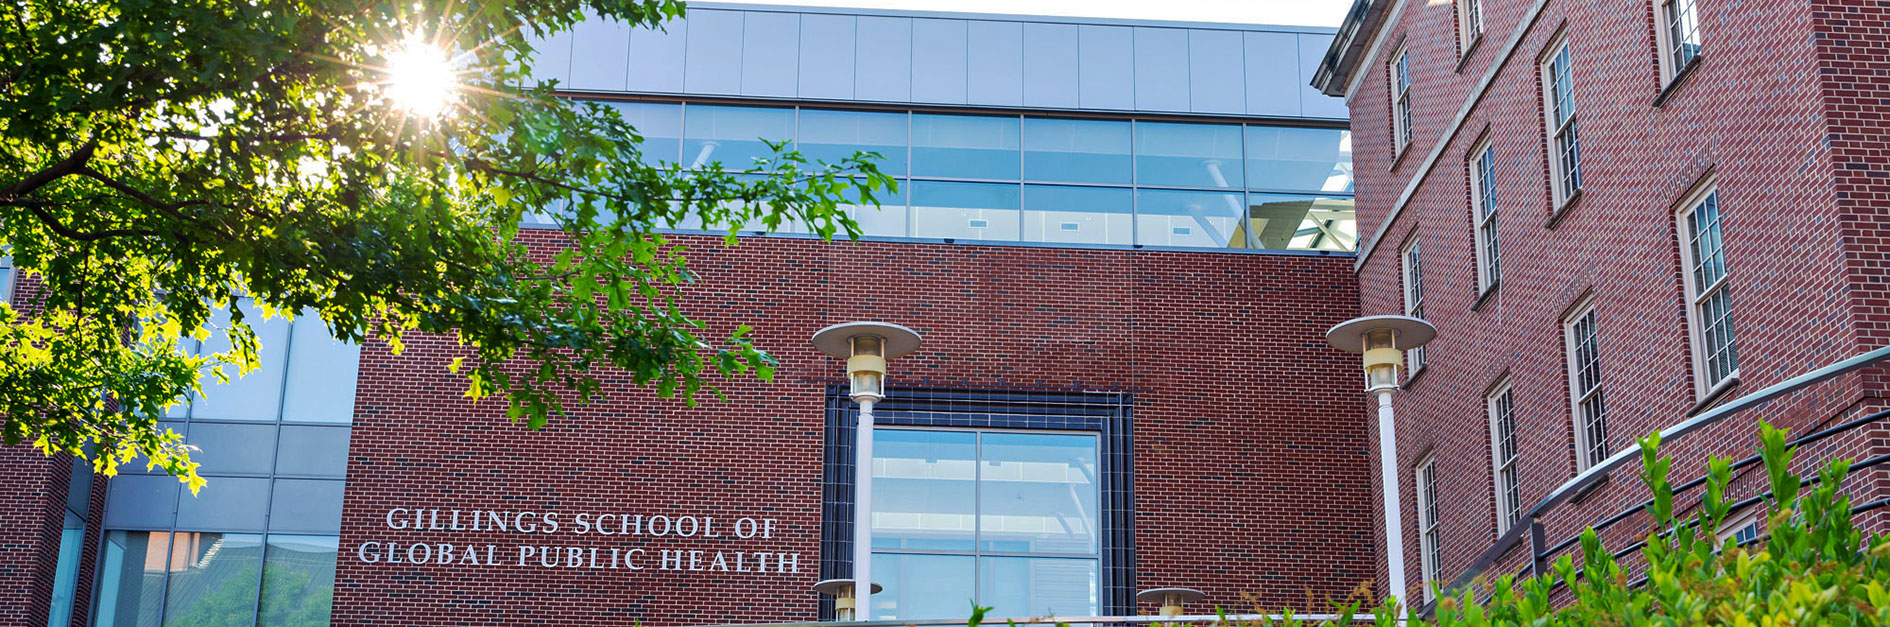
\includegraphics[width=0.9\linewidth]{images/unc.jpeg}
    \end{center}
    \textbf{Data:} \colorbox{ddefblue}{This is a picture of UNC} \\\vspace{1mm} The school we go to. \\\vspace{3mm}
    \textbf{Outcomes:} \colorbox{ddefblue}{Hopefully graduation from UNC.}\\
\begin{itemize}
    \item[\textendash] Please don't forget to change this picture.
\end{itemize}
%\vspace{-3mm}
    
\end{frame}
\begin{frame}
    \frametitle{Main Concepts}
    \framesubtitle{Topics we love in this lab}
    
    \begin{minipage}{0.5\textwidth}
        \setbeamertemplate{enumerate items}{\raisebox{-0.2em}{\scalebox{1.3}{\circled{\color{white}\insertenumlabel}}}}
        \begin{enumerate}
            \itemsep1.3em
            \item ITR Estimation (Decision Support)
            \item SMARTs
            \item Prescriptive variable selection
        \end{enumerate}
    \end{minipage} \hfill
    \begin{minipage}{0.49\textwidth}
        \begin{figure}
            
\includegraphics[width=1.0\linewidth]{images/big_data_image.jpg}
        \end{figure}
    \end{minipage}
    
\end{frame}

\begin{frame}
    \frametitle{Key Features}
    
    \dbox{
    \setbeamertemplate{itemize items}{\raisebox{-0.2em}{\scalebox{1.2}{\circledmark{}}}}
    \begin{itemize}
        \itemsep1.3em
        \item Checkmarks are really cool
        \item List things nicely
        \item Make the bulleted list look fancy
    \end{itemize}
    }
\end{frame}

\begin{frame}{Takeaways}
    \vspace{3mm}
%\setlength\itemsep{1.3em}
\setbeamertemplate{enumerate items}{\raisebox{-0.1em}{\scalebox{1.3}{\circled{\color{white}\insertenumlabel}}}}
\begin{enumerate}[<+->]
    \itemsep1.5em
    \item This is what your audience will takeaway
    \item Takeaway 2 (example of how to make bullet points appear)
    \item Another one
\end{enumerate} 
\end{frame}
\begin{frame}[plain,noframenumbering]{Acknowledgements}
\begin{columns}[T]
\begin{column}{.5\textwidth}
\vspace{2mm}
My dissertation advisors:

    \begin{itemize}\setlength\itemsep{0.1em}
        \item Insert advisor here, Ph.D.
        \item Insert advisor here, Ph.D.
    \end{itemize}\leavevmode\newline
    Collaborators:
    %\vspace{1em}
        \begin{itemize}\setlength\itemsep{0.1em}
        \item Insert collaborators here, Ph.D.
        \item Insert collaborators here, M.D.
        \item Insert collaborators here
        \end{itemize}
    \leavevmode\newline
    PHAIR Lab members.\leavevmode\newline
    Insert funding sources here
\end{column}
\begin{column}{.5\textwidth}
    \begin{center}
        \vspace{-4mm}
        
\includegraphics[width=.8\linewidth]{images/kosoroklablogo_withtext.png}
    \end{center}
\end{column}%
\end{columns}
\end{frame}

\appendix

{
    \setbeamercolor{background canvas}{bg=VKblue}
    \frame[plain,noframenumbering]{
        \vspace{2cm}
        \usebeamerfont{title}\usebeamercolor[fg]{title} \textbf{{\Huge Thank you!}} \\
        \usebeamerfont{author}\usebeamercolor[fg]{author}
        \vfill
        \vspace*{5mm}
        %\insertauthor, Ph.D. \\
        You can contact me at: \textbf{name@live.unc.edu}
    }
}

{
\setbeamercolor{background canvas}{bg=VKblue}
\begin{frame}[plain,noframenumbering]
\vspace{1cm}
\usebeamerfont{title}\usebeamercolor[fg]{title} \textbf{{\Huge Appendix}}
\end{frame}
}

\begin{frame}{\hypertarget{appendix:notation}{Appendix: Notation (Expanded)}}

\begin{enumerate}\itemsep4mm
    \item Math can go here: $m(\bm{X}) = 1 + 10X_1$.
    \item More math here.
    \item Another point here.
\end{enumerate}
\vspace{4mm}
\begin{center}
    \hyperlink{notation}{\textcolor{blue}{{\small (Back to main notation slide.)}}}
\end{center}
    
\end{frame}

\end{document} 